\documentclass{beamer}
\usepackage[utf8]{inputenc} % Obsługa kodowania UTF-8
\usepackage[T1]{fontenc}    % Poprawna obsługa czcionek
\usepackage[polish, english]{babel} % Obsługa języka polskiego i angielskiego
\usepackage{graphicx} % Dodawanie grafik
\usepackage{hyperref} % Linki w dokumencie
\usepackage{xcolor} % Kolory

% Tytuł i autorzy
\title{Analiza danych przestrzennych - Modelowanie i wizualizacja}
\author{Marcin Samojluk, Gabriel Rączkowski}
\date{\today}

% Definicja kolorów dla tytułów
\definecolor{darkblue}{rgb}{0.0, 0.0, 0.5}

% Zmiana koloru tła tytułów slajdów
\setbeamercolor{frametitle}{bg=darkblue, fg=white} % Ciężki niebieski i biały tekst dla tytułów

\begin{document}

% Strona tytułowa
\frame{\titlepage}

% Spis treści
\begin{frame}{Plan prezentacji}
    \tableofcontents
\end{frame}

% Wstęp
\section{Wstęp}
\begin{frame}{Wstęp}
    \begin{itemize}
        \item Celem projektu jest analiza danych przestrzennych na wybranym obszarze.
        \item Dane pochodzą z narzędzi:
        \begin{itemize}
            \item QGIS - analiza danych przestrzennych.
            \item GEBCO - podkład topograficzny.
            \item ParaView - wizualizacja i analiza trójwymiarowa.
        \end{itemize}
        \item Analizowane parametry:
        \begin{itemize}
            \item Azymuty i kąty nachylenia powierzchni (Dip Direction, Dip Angle).
            \item Grupowanie trójkątów w przestrzeni za pomocą algorytmu k-średnich.
        \end{itemize}
    \end{itemize}
\end{frame}

% Mapa topograficzna
\section{Mapa topograficzna}
\begin{frame}{Mapa topograficzna}
    \begin{itemize}
        \item Podkład topograficzny przygotowano za pomocą wtyczki OpenLayersPlugin w QGIS.
        \item Obszar danych został zaznaczony w GEBCO, a następnie naniesiony na mapę.
    \end{itemize}
    \begin{figure}
        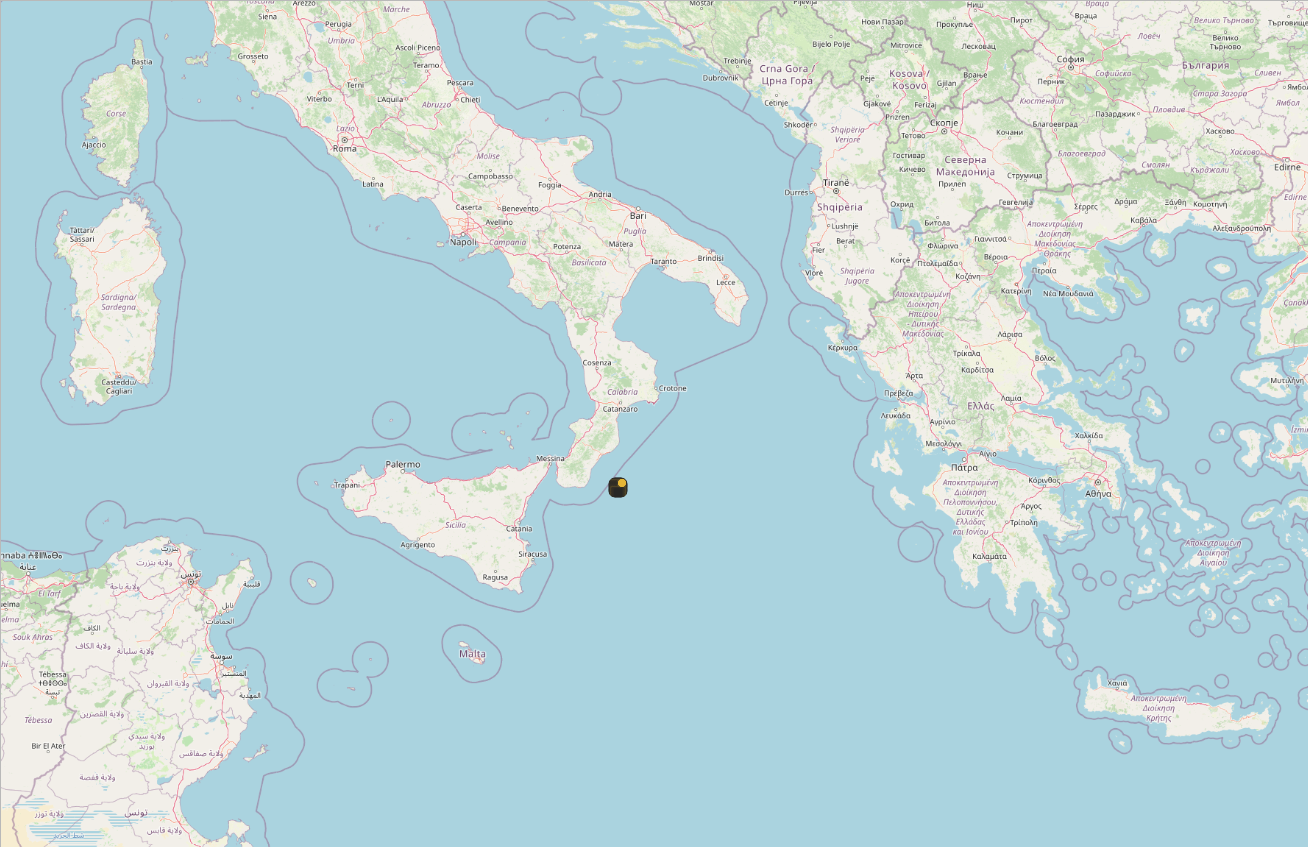
\includegraphics[width=0.7\textwidth]{topograf.png}
        \caption{Mapa topograficzna z zaznaczonym obszarem.}
    \end{figure}
\end{frame}

% Mapa azymutów (Dip Direction)
\section{Mapa azymutów (Dip Direction)}
\begin{frame}{Mapa azymutów (Dip Direction)}
    \begin{itemize}
        \item Przygotowano w QGIS z użyciem danych interpolowanych.
        \item Analizowano nachylenie, ekspozycję oraz azymuty powierzchni.
    \end{itemize}
    \begin{figure}
        \centering
        % Pierwszy obraz
        \begin{minipage}{0.3\textwidth}
            \centering
            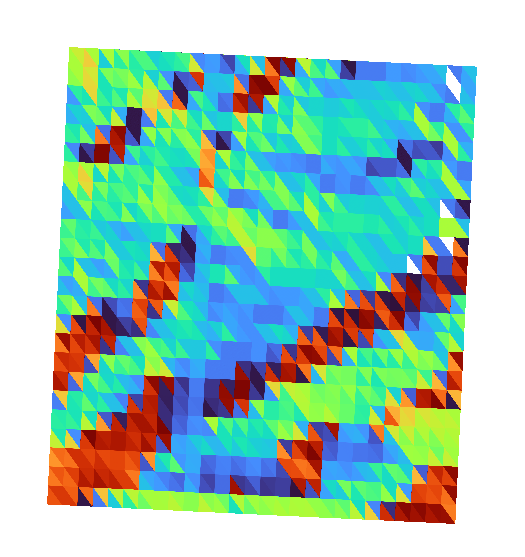
\includegraphics[width=\textwidth]{Eks.png}
            \caption{Ekspozycja (Exposure).}
        \end{minipage}
        \hspace{0.2cm} % Odstęp między obrazkami
        % Drugi obraz
        \begin{minipage}{0.3\textwidth}
            \centering
            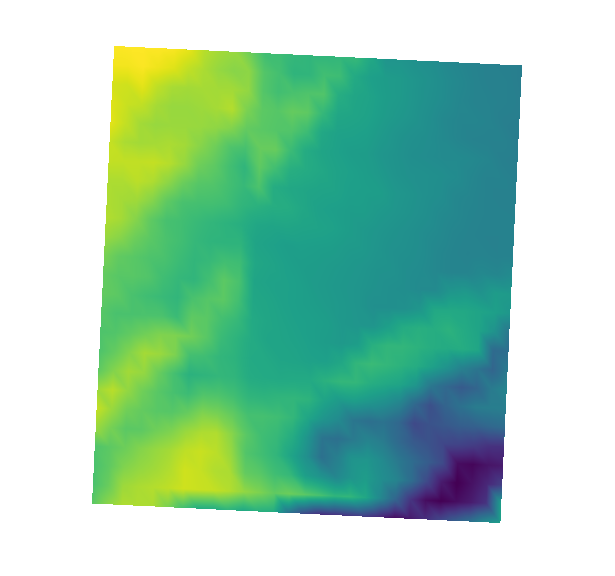
\includegraphics[width=\textwidth]{Inter.png}
            \caption{Interpolowane dane powierzchniowe.}
        \end{minipage}
        \hspace{0.2cm} % Odstęp między obrazkami
        % Trzeci obraz
        \begin{minipage}{0.3\textwidth}
            \centering
            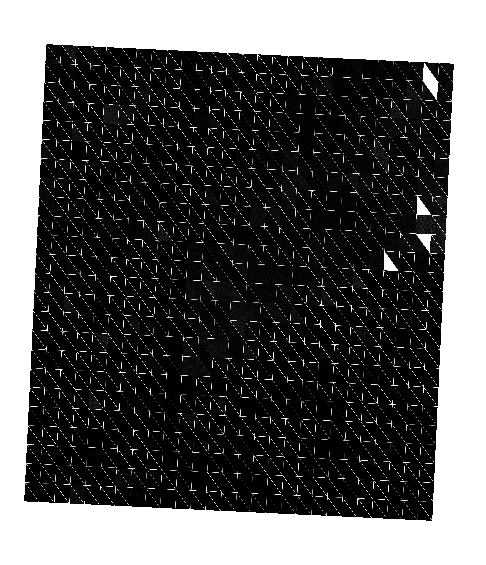
\includegraphics[width=\textwidth]{nach.png}
            \caption{Nachylenie powierzchni (Dip Angle).}
        \end{minipage}
    \end{figure}
\end{frame}

% Grupowanie trójkątów - X_N, Y_N, Z_N
\section{Grupowanie trójkątów - X\_N, Y\_N, Z\_N}
\begin{frame}{Grupowanie trójkątów - X\_N, Y\_N, Z\_N}
    \begin{itemize}
        \item Grupowanie przeprowadzono za pomocą algorytmu k-średnich.
        \item Analiza dla kolumn $X_N$, $Y_N$, $Z_N$.
        \item Wyniki wizualizowane w stereonete z zaznaczonymi środkami skupień.
    \end{itemize}
    \begin{figure}
        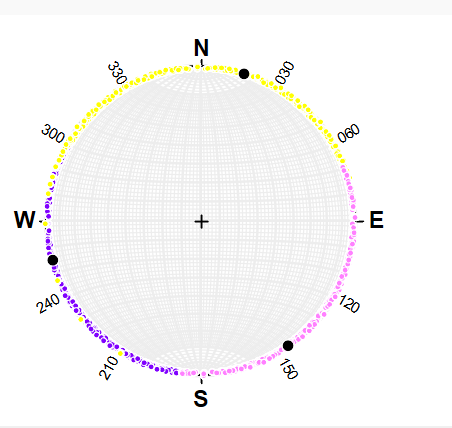
\includegraphics[scale=0.5]{X_N.png}
        \caption{Stereonet z zaznaczonymi środkami skupień dla $X_N$, $Y_N$, $Z_N$.}
    \end{figure}
\end{frame}

% Grupowanie trójkątów - X_D, Y_D, Z_D
\section{Grupowanie trójkątów - X\_D, Y\_D, Z\_D}
\begin{frame}{Grupowanie trójkątów - X\_D, Y\_D, Z\_D}
    \begin{itemize}
        \item Grupowanie przeprowadzono analogicznie jak dla $X_N$, $Y_N$, $Z_N$.
        \item Analiza dla kolumn $X_D$, $Y_D$, $Z_D$.
    \end{itemize}
    \begin{figure}
        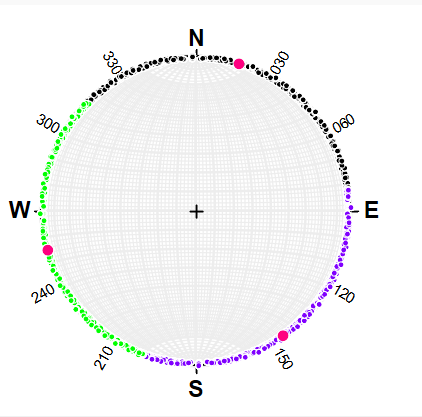
\includegraphics[scale=0.5]{X_D.png}
        \caption{Stereonet z zaznaczonymi środkami skupień dla $X_D$, $Y_D$, $Z_D$.}
    \end{figure}
\end{frame}





% Slajd z tabelami punktów skupień
\section{Tabele punktów skupień}
\begin{frame}{Tabele punktów skupień}
    \begin{itemize}
        \item Tabele przedstawiają wartości punktów skupień wyznaczonych w analizie.
        \item Zestawiono wartości przed i po przefiltrowaniu.
    \end{itemize}
    \begin{figure}
        \centering
        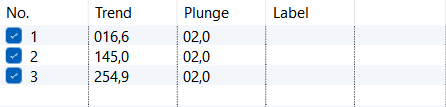
\includegraphics[width=0.45\textwidth]{X_N_measure.png}
        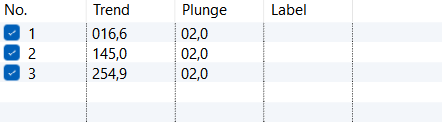
\includegraphics[width=0.45\textwidth]{X_D_measure.png}
        \caption{Tabela punktów skupień: X\_N (lewo) i X\_D (prawo).}
    \end{figure}
\end{frame}


% Slajd z kodem filtrowania i wizualizacji ggplot
\section{Kod filtrowania i wizualizacji w R}
\begin{frame}{Kod filtrowania i wizualizacji w R}
    \begin{block}{Filtrowanie danych}
        \texttt{filter\_tab1 <- dplyr::filter(tab1, Dip\_ang > 0 \& Dip\_ang < 91,}\\
        \texttt{X\_N > -0.05 \& X\_N < 0.05, Y\_N > -0.05 \& Y\_N < 0.05)}
    \end{block}
    \begin{block}{Kod ggplot dla oryginalnych danych}
        \texttt{ggplot(data=tab1, aes(x = Y\_C, y = X\_C, color = Dip\_ang )) + geom\_point()}
    \end{block}
    \begin{block}{Kod ggplot dla przefiltrowanych danych}
        \texttt{ggplot(data=filter\_tab1, aes(x = Y\_C, y = X\_C, color = Dip\_ang )) + geom\_point()}
    \end{block}
    \begin{itemize}
        \item Filtrowanie danych pozwala na wybór punktów spełniających określone kryteria.
        \item Wizualizacja umożliwia analizę rozkładu danych przed i po przefiltrowaniu.
    \end{itemize}
\end{frame}


% Slajd z przefiltrowanymi punktami
\section{Przefiltrowane punkty}
\begin{frame}{Przefiltrowane punkty}
    \begin{itemize}
        \item Wykresy przedstawiają dane przed i po przefiltrowaniu.
        \item Kolor punktów odpowiada wartości kąta nachylenia (\textit{Dip Angle}).
    \end{itemize}
    \begin{figure}
        \centering
        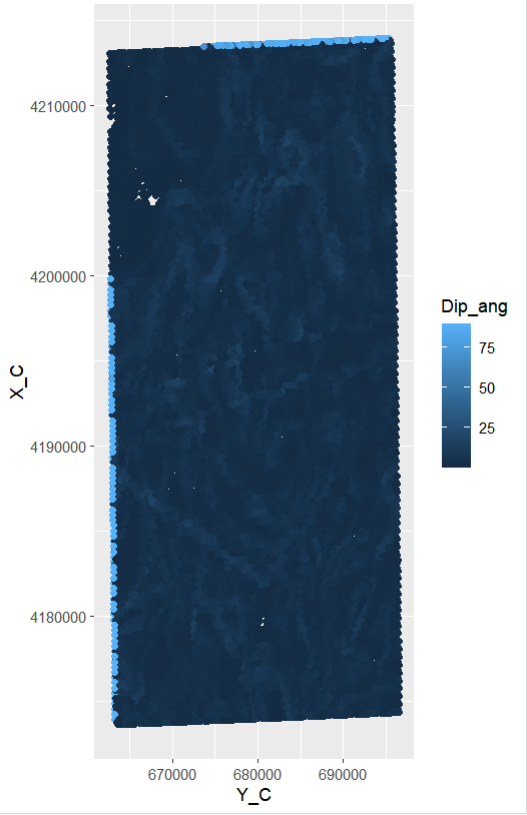
\includegraphics[width=0.45\textwidth]{before.png}
        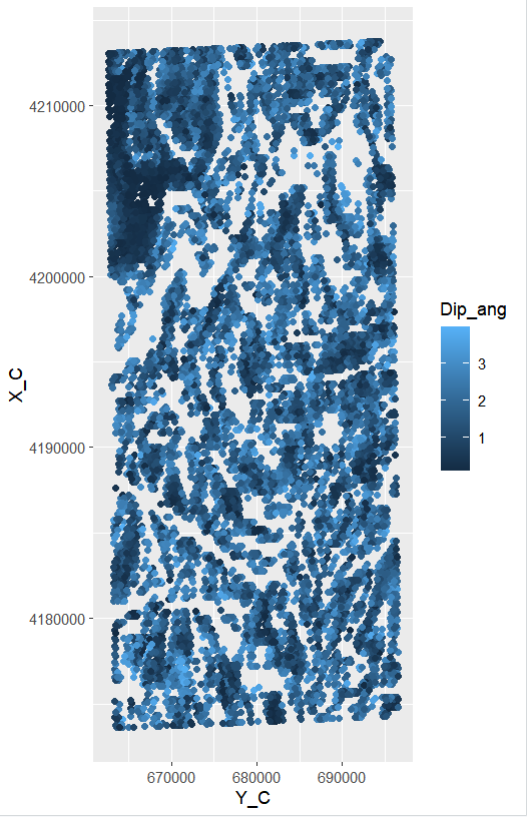
\includegraphics[width=0.45\textwidth]{after.png}
        \caption{Punkty przed przefiltrowaniem (lewo) i po przefiltrowaniu (prawo).}
    \end{figure}
\end{frame}



% Sekcja: Mapa geomorfonów
\section{Mapa geomorfonów}

% Slajd z opisem mapy geomorfonów
\begin{frame}{Mapa geomorfonów - Opis}
    \begin{itemize}
        \item Mapa geomorfonów przedstawia klasyfikację geomorficzną analizowanego obszaru.
        \item Wartości geomorfonów zostały przypisane na podstawie analizy zmienności terenu, uwzględniając nachylenie, azymut i krzywiznę powierzchni.
        \item Kolorystyka na mapie pokazuje różne typy ukształtowania terenu, w tym wzgórza, doliny oraz płaskie obszary.
        \item Analiza geomorfonów jest przydatna w badaniach geomorfologicznych, planowaniu przestrzennym i analizach środowiskowych.
    \end{itemize}
\end{frame}

% Slajd z mapą geomorfonów

\section{Mapa geomorfonów}
\begin{frame}{Mapa geomorfonów - Wizualizacja}
    \begin{figure}
        \centering
        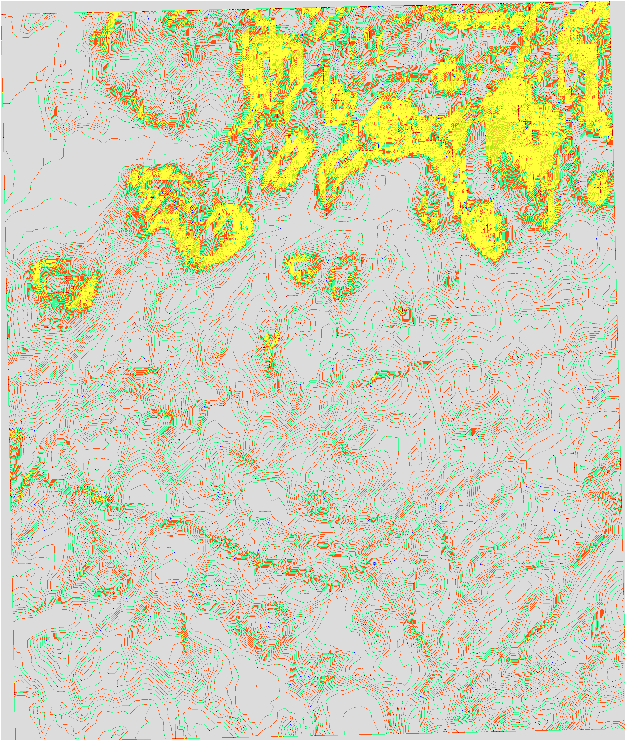
\includegraphics[width=0.5\textwidth]{geo.png} % Ścieżka do pliku z mapą
        \caption{Mapa geomorfonów - Klasyfikacja geomorficzna obszaru.}
    \end{figure}
\end{frame}






% Podsumowanie i wnioski
\section{Podsumowanie i wnioski}
\begin{frame}{Podsumowanie i wnioski}
    \begin{itemize}
        \item Przeanalizowano dane przestrzenne i dokonano wizualizacji za pomocą stereonetu.
        \item Wyniki wskazują na różnice w rozkładzie azymutów dla różnych grup trójkątów.
        \item Możliwe rozszerzenia analizy:
        \begin{itemize}
            \item Dalsza integracja z modelami 3D w ParaView.
            \item Analiza błędów i ich wpływu na wyniki.
        \end{itemize}
        \item Wnioski mogą być przydatne w analizach geologicznych i geomorfologicznych.
    \end{itemize}
\end{frame}

% Bibliografia
\section{Bibliografia}
\begin{frame}{Bibliografia}
    \begin{itemize}
        \item GEBCO - \url{https://www.gebco.net/}
        \item QGIS - \url{https://qgis.org/}
        \item ParaView - \url{https://www.paraview.org/}
        \item Dokumentacja Stereonet - dostępna w programie.
        
    \end{itemize}
\end{frame}

\end{document}
